If one searches for an ellipse's inscribed 4-gon of maximal perimeter, one finds the family of $N=4$ orbits which are all parallelograms \cite{connes07}. Their tangential polygons (tangent at the ellipse) are rectangles, and their vertices describe a circular locus, known as Monge's Orthoptic Circle \cite{mw}, Figure~\ref{fig:monge-orthoptic}:

Close observation of the above provided us with invaluable clues with which to generalize $N=3$ invariants to $N>3$ orbits. Namely:

\begin{itemize}
    \item Stationary Circle: The orthoptic locus is a stationary circle.
    \item Null Sum of Cosines: The polygon formed by the four tangency points is a parallelogram so the sum of its cosines is therefore zero.
    \item Null Product of Cosines: The Tangential Polygon is a rectangle and therefore the product of its cosines is zero.
    \item Mittenpunkt: The lines connecting the Tangential Polygon's vertices to the parallelogram midpoints concur at the Ellipse's center.
\end{itemize}

\subsection{$N>3$ Stationary Point}

For an $N=3$ orbit, the Mittenpunkt is where lines drawn from each Excenter through the sides' midpoints meet. As shown in Figure~\ref{fig:gen-mitten}, lines drawn from each vertex of the Tangential Polygon through the midpoint of the corresponding orbit side will meet at the stationary center of the Billiard. The same Affine Transform argument of Figure~\ref{fig:mitten-proof} can be used here, so we can state:

\begin{observation}
Consider an $N\geq{3}$ orbit family. The point of concurrence of lines from tangential vertices tangential through the orbit side midpoints is stationary at the center of the Billiard.
\end{observation}

\begin{figure}
    \centering
    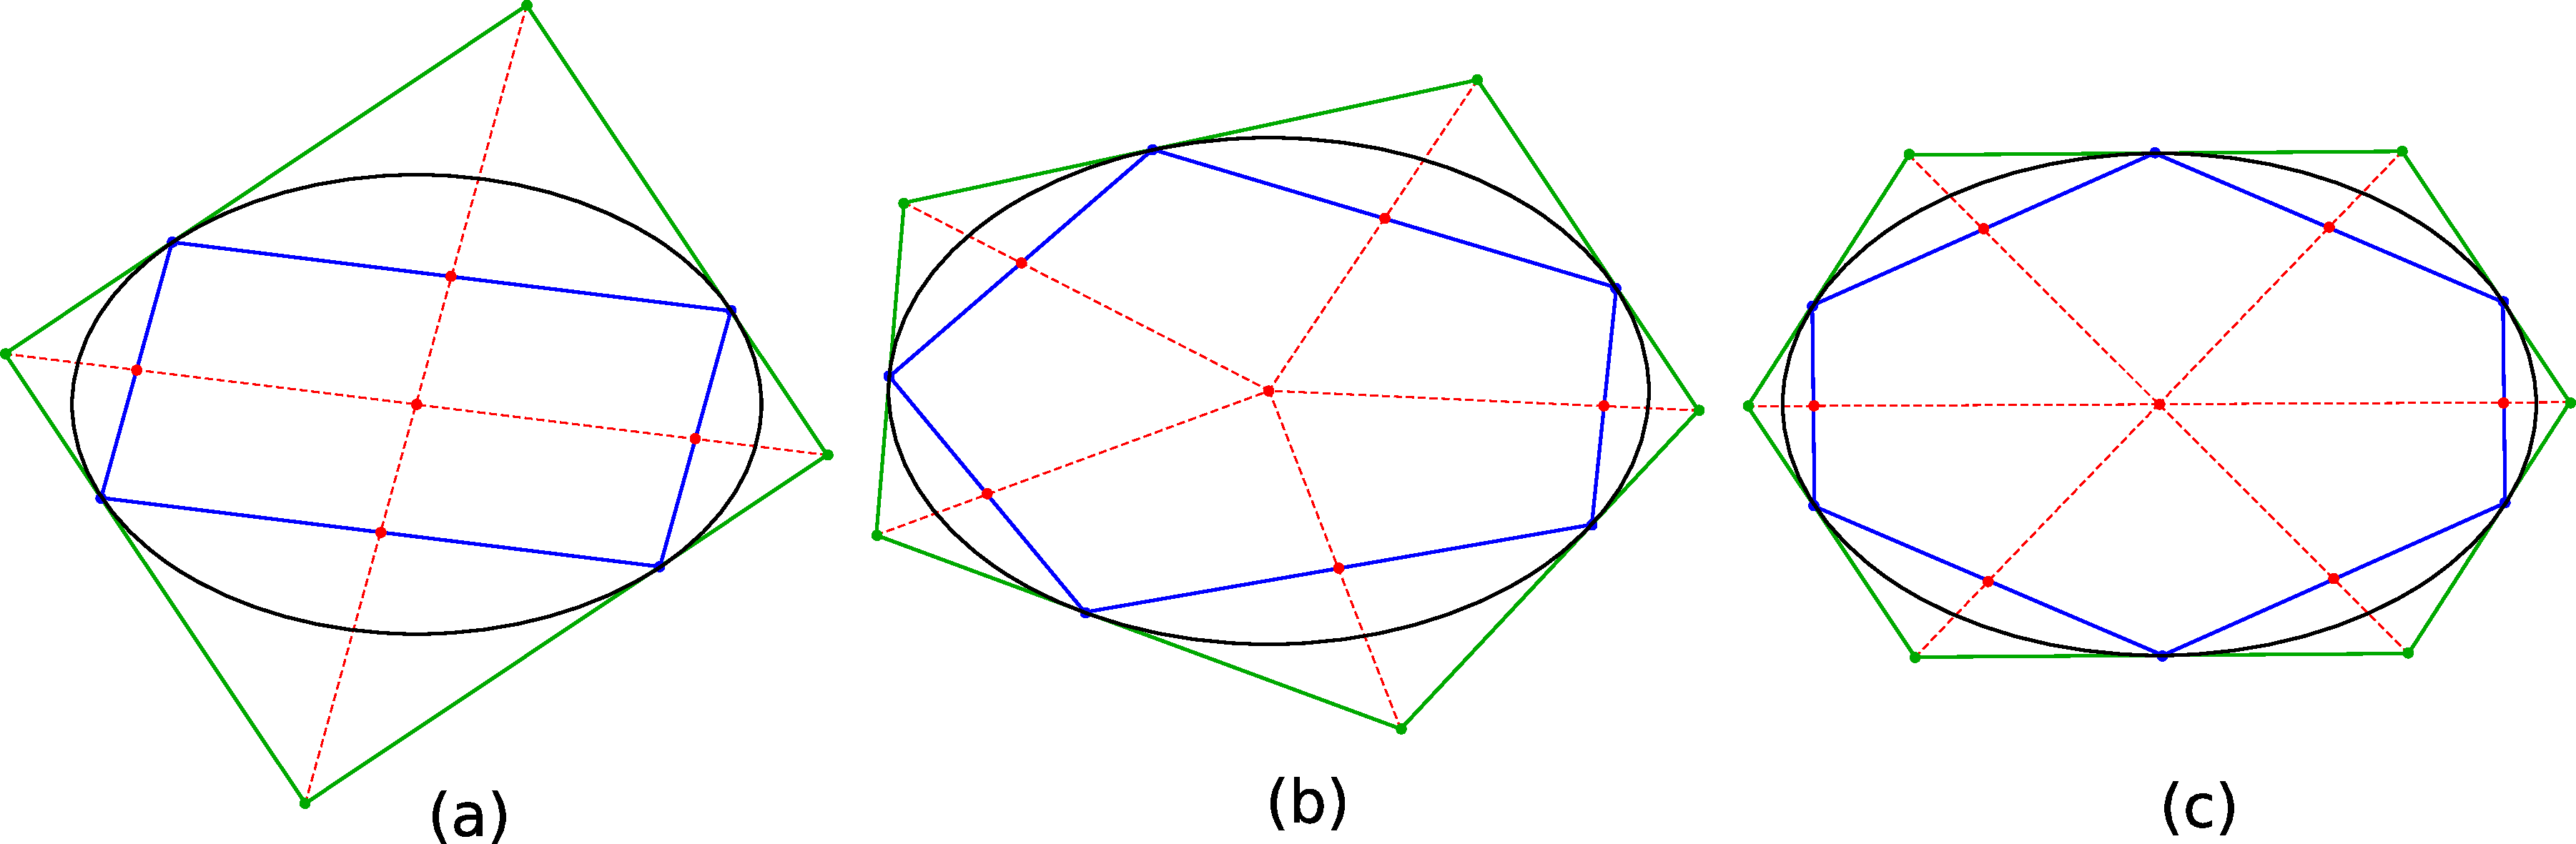
\includegraphics[width=\textwidth]{pics/0150_gener_mitten.pdf}
    \caption{Lines drawn from the vertices of an $N>3$ orbit's Tangential Polygon passing through the midpoint of the corresponding orbit sides meet at the stationary center of the Billiard.}
    \label{fig:gen-mitten}
\end{figure}

\subsection{$N>3$ Cosine Sum and Product}

The fact that both $N=3$ and $N=4$ conserve cosine sum, suggests $N>4$ might as well, and this was first confirmed numerically for $N=5,..30$ non-intersecting orbits at various Billiard aspect ratios. Figure~\ref{fig:gen-cos-sum-n45} shows cosine curves adding to a constant for $N=4,5$ with $a=1.5$.

The following elegant proof has been kindly contributed \cite{sergei19_private_meromorphic}. Using Equation~\ref{eqn:joachim} the half-angle cosine in terms of momentum and length of gradient, and then with $\cos{t}=2\cos(t/2)^2-1$ write an expression for the sum of full-angle cosines:

\begin{eqnarray}
\cos\frac{\theta_i}{2} & = & \frac{\gamma}{|\nabla{f_i}|}\\
\sum_{i=1}^{N}{\cos\theta_i} & = & 2\,{\gamma}\sum_{i=1}^{N}\frac{1}{|\nabla{f_i}|^2}-N
\label{eqn:cosine-sum}
\end{eqnarray}

\noindent where $f_i=f(P_i)$. Then complexify the space and show that the poles of Equation~\ref{eqn:cosine-sum} on the elliptic curve covering the conic cancel each other. So one has a pole-free meromorphic function, hence a constant.

\begin{theorem}
The sum of cosines is conserved for non-intersecting orbits, $\forall{N}$.
\end{theorem}

\begin{figure}[H]
    \centering
    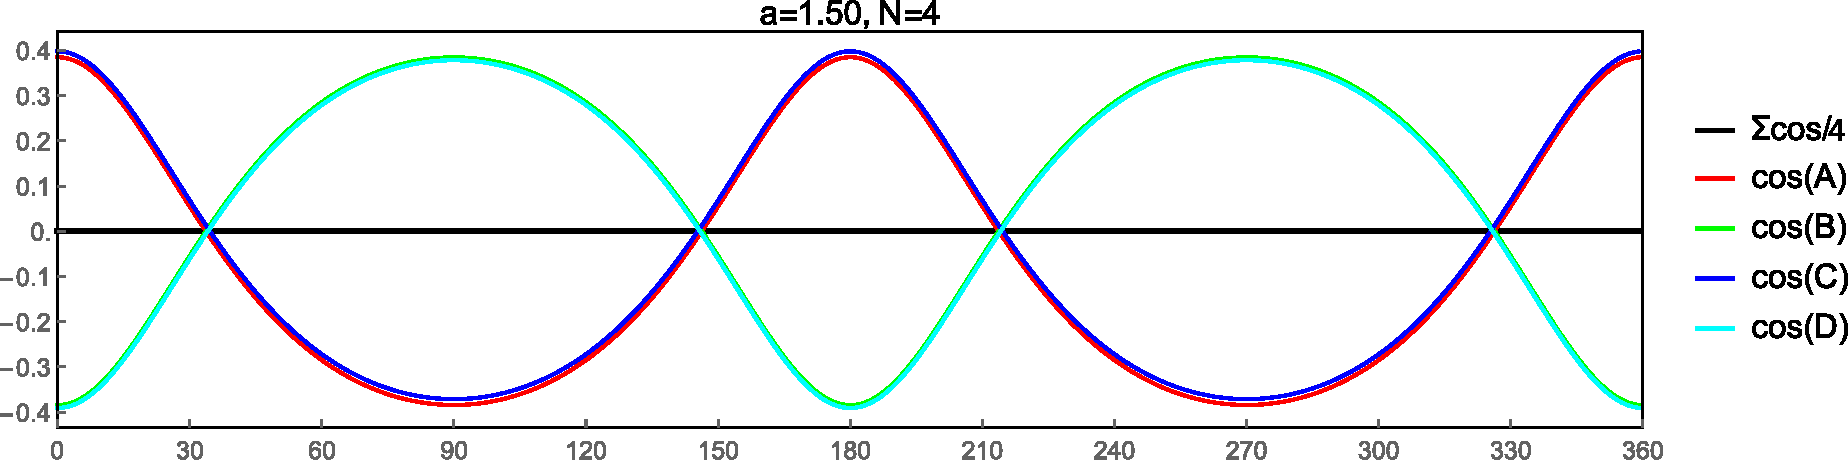
\includegraphics[width=\textwidth]{pics/0091_cosine_sum_n4.pdf}
    %
    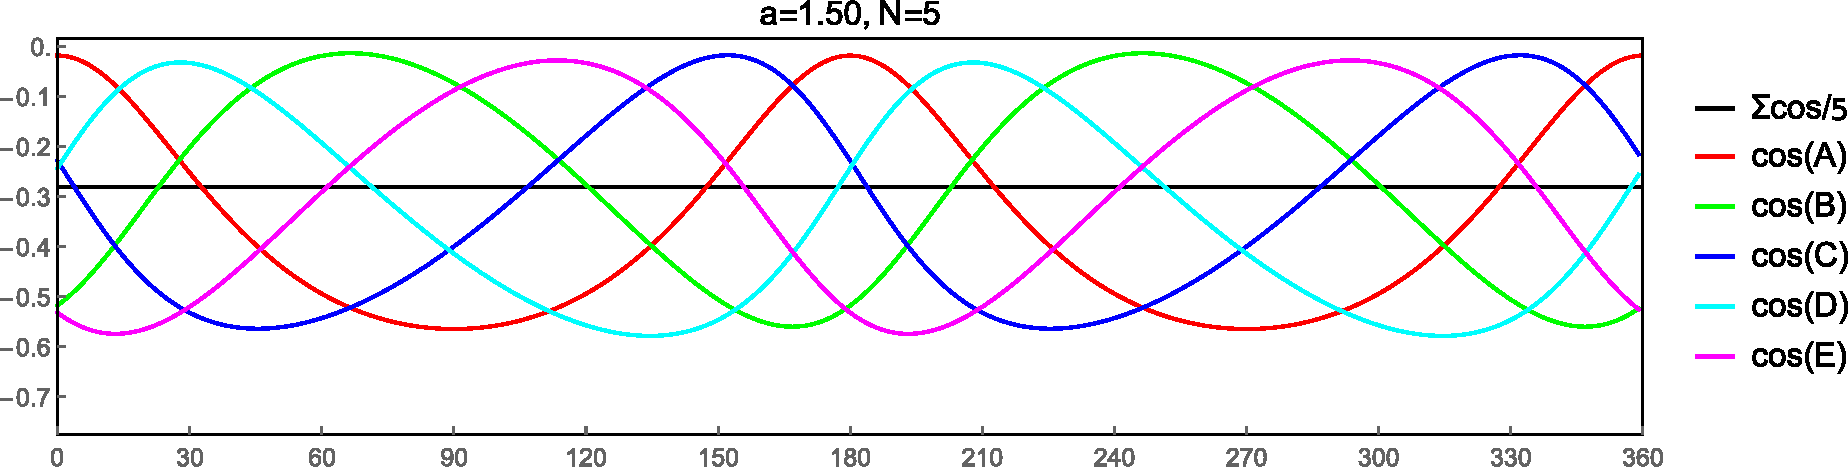
\includegraphics[width=\textwidth]{pics/0092_cosine_sum_n5.pdf}
    \caption{Individual cosine values are shown for the $N=4$ (top) and $N=5$ (bottom) family of orbits, $a=1.5$, vs. the parameter of a leader vertex. $N=4$ orbits are parallelograms, so opposite angles are supplementary and cosine curves are superimposed and symmetric, adding to zero. In the more asymmtric $N=5$ case, the 5 cosines still add to a constant value (black line at the bottom of the graph).}
    \label{fig:gen-cos-sum-n45}
\end{figure}

\begin{figure}[H]
    \centering
    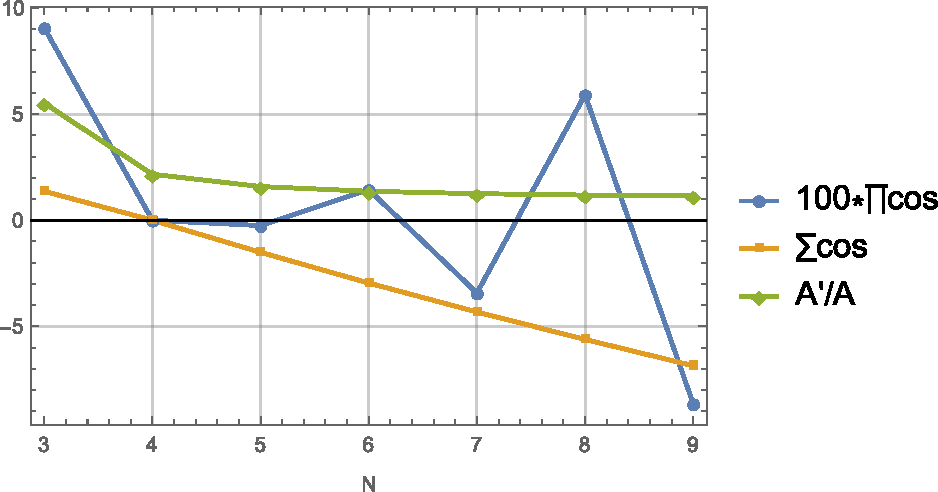
\includegraphics[width=\textwidth]{pics/0160_gener_prod_sum_area.pdf}
    \caption{Constant orbit cosine sum, tangential polygon cosine product (the latter is multiplied by a 100 to be visible), and tangential-to-orbit area ratio vs. $N$ for $a=1.5$.}
    \label{fig:gen-prod-sum}
\end{figure}

Similarly, since both $N=3$ and $N=4$ conserve the product of their Excentral/Tangential cosines, we verify numerically that $N=5,..30$ non-intersecting orbits at various aspect ratios also conserve this quantity. A proof to which (with similar techniques) has been kindly shared with us \cite{sergei19_private_meromorphic}.

\begin{theorem}
The product of cosines for non-intersecting orbits for {\em any} $N$ is conserved.
\end{theorem}

When trajectories are not closed, the sum of their cosines (resp. product of their excentral cosines) may be unbounded. One can then talk about the arithmetic mean (resp. geometric mean) of cosines for open trajectories (resp. their external tangents). In the Appendix we show how special spatial integrals can compute them, showing perfect match with the case when trajectories are closed orbits.

\subsection{Area Ratio for $N>3$}

For $N=3$ the Excentral-to-Orbit area ratio is conserved, however, we can easily check numerically that $N=4$ does not preserve the ratio of its rectangular Tangential-to-Orbit polygons.

Proceeding to $N>4$ we verify that only odd $N$ preserve area ratio, a fact which has been subsequently formally proven \cite{sergei19_private_meromorphic}. 
Figure~\ref{fig:gen-prod-sum} shows cosine sum, cosine product, and area ratio invariants for $N=3,4,\ldots,9$.

\begin{theorem}
The ratio of areas between Tangential Polygon and Non-Self-Intersecting Orbit is conserved for all odd $N$.
\end{theorem}

\subsection{Stationary $N>4$ Circles}

For the $N=3$ case,  Figure~\ref{fig:cosine_hexagon}(b), the locus of the intersection of an edge in the Excentral Triangle with an alternate edge reflected about the Billiard center is a stationary circle. For $N=4$ we have Monge's Orthoptic Circle. Can these two constructions be harmonized and extended to $N>4$? Indeed it can, in this surprising way:

\begin{theorem}
Let $O$ be the center of the Billiard. The locus of the intersection of an edge of the Tangential Polygon with the reflection of the next tangential edge about $O$ is a stationary circle centered on $O$. Its radius is $r^*=1/\gamma$, i.e., the inverse of angular momentum.
\end{theorem}

\noindent {\bf Proof} \cite{sergei19_private_circles}: Let $f$ be as in Equation~\ref{eqn:f}. $f_X$ represent $f(X)$. Consider two consecutive vertices $P$ and $Q$ of the orbit. Then:

\begin{itemize}
\item By momentum conservation $\hat{v}.\nabla f_P= -\hat{v}.\nabla f_Q=\gamma$. So we have:

\begin{equation}
    \hat{v}.\left(\nabla{f_P} + \nabla{f_Q}\right)=0
    \label{eqn:sum-nablas}
\end{equation}

\item Since $\nabla{f_P}$ (resp. $\nabla{f_Q}$) is normal to the ellipse at $P$ (resp.  $Q$), a point $z$ on the tangent line at $P$ (resp. $-Q$) is given by $z.\nabla{f_P}=1$ (resp. $z.\nabla{f_Q}=-1$).
\item Let $z$ be where both lines intersect, $z.\left(\nabla{f_P}+{\nabla} f_Q\right)=0$.

\item It follows from Equation~\ref{eqn:sum-nablas} that $z$ is proportional to $\hat{v}$.

\item Since $\hat{v}.\nabla{f_P}=\gamma$ and $z.\nabla{f_P}=1$, we have $z = \hat{v}/\gamma$.
\item That is, $z$ lies on the circle of radius $1/\gamma$.\qed
\end{itemize}

\noindent The radius of the stationary circle is plotted against the aspect ratio of the Billiard for a range of $N$ in Figure~\ref{fig:stationary-radius-vs-a}. The stationary circle is shown around various $N$ in  Figure~\ref{fig:gen-circ-grid} .

\begin{figure}
    \centering
    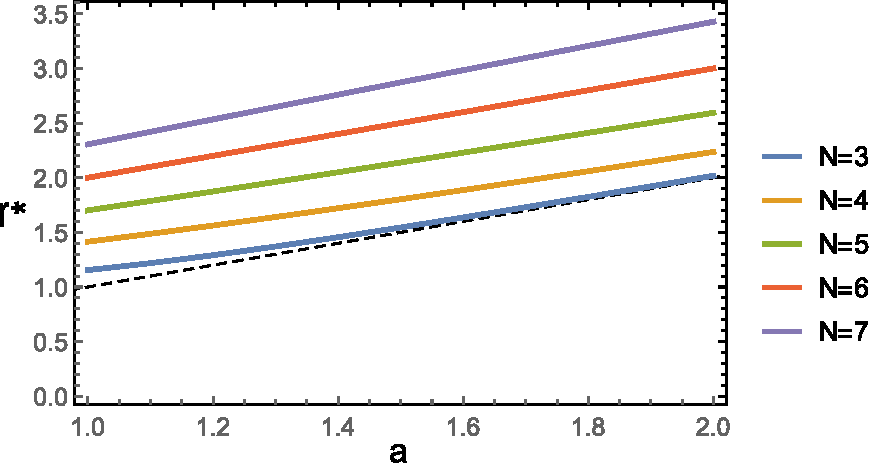
\includegraphics[width=.75\textwidth]{pics/0190_rstar.pdf}
    \caption{Radius of stationary circle vs $a$, for different values of $N$. A $x=y$ dashed line is drawn to show that for $N=3$, $r^*>a$.}
    \label{fig:stationary-radius-vs-a}
\end{figure}

\begin{figure}[H]
    \centering
    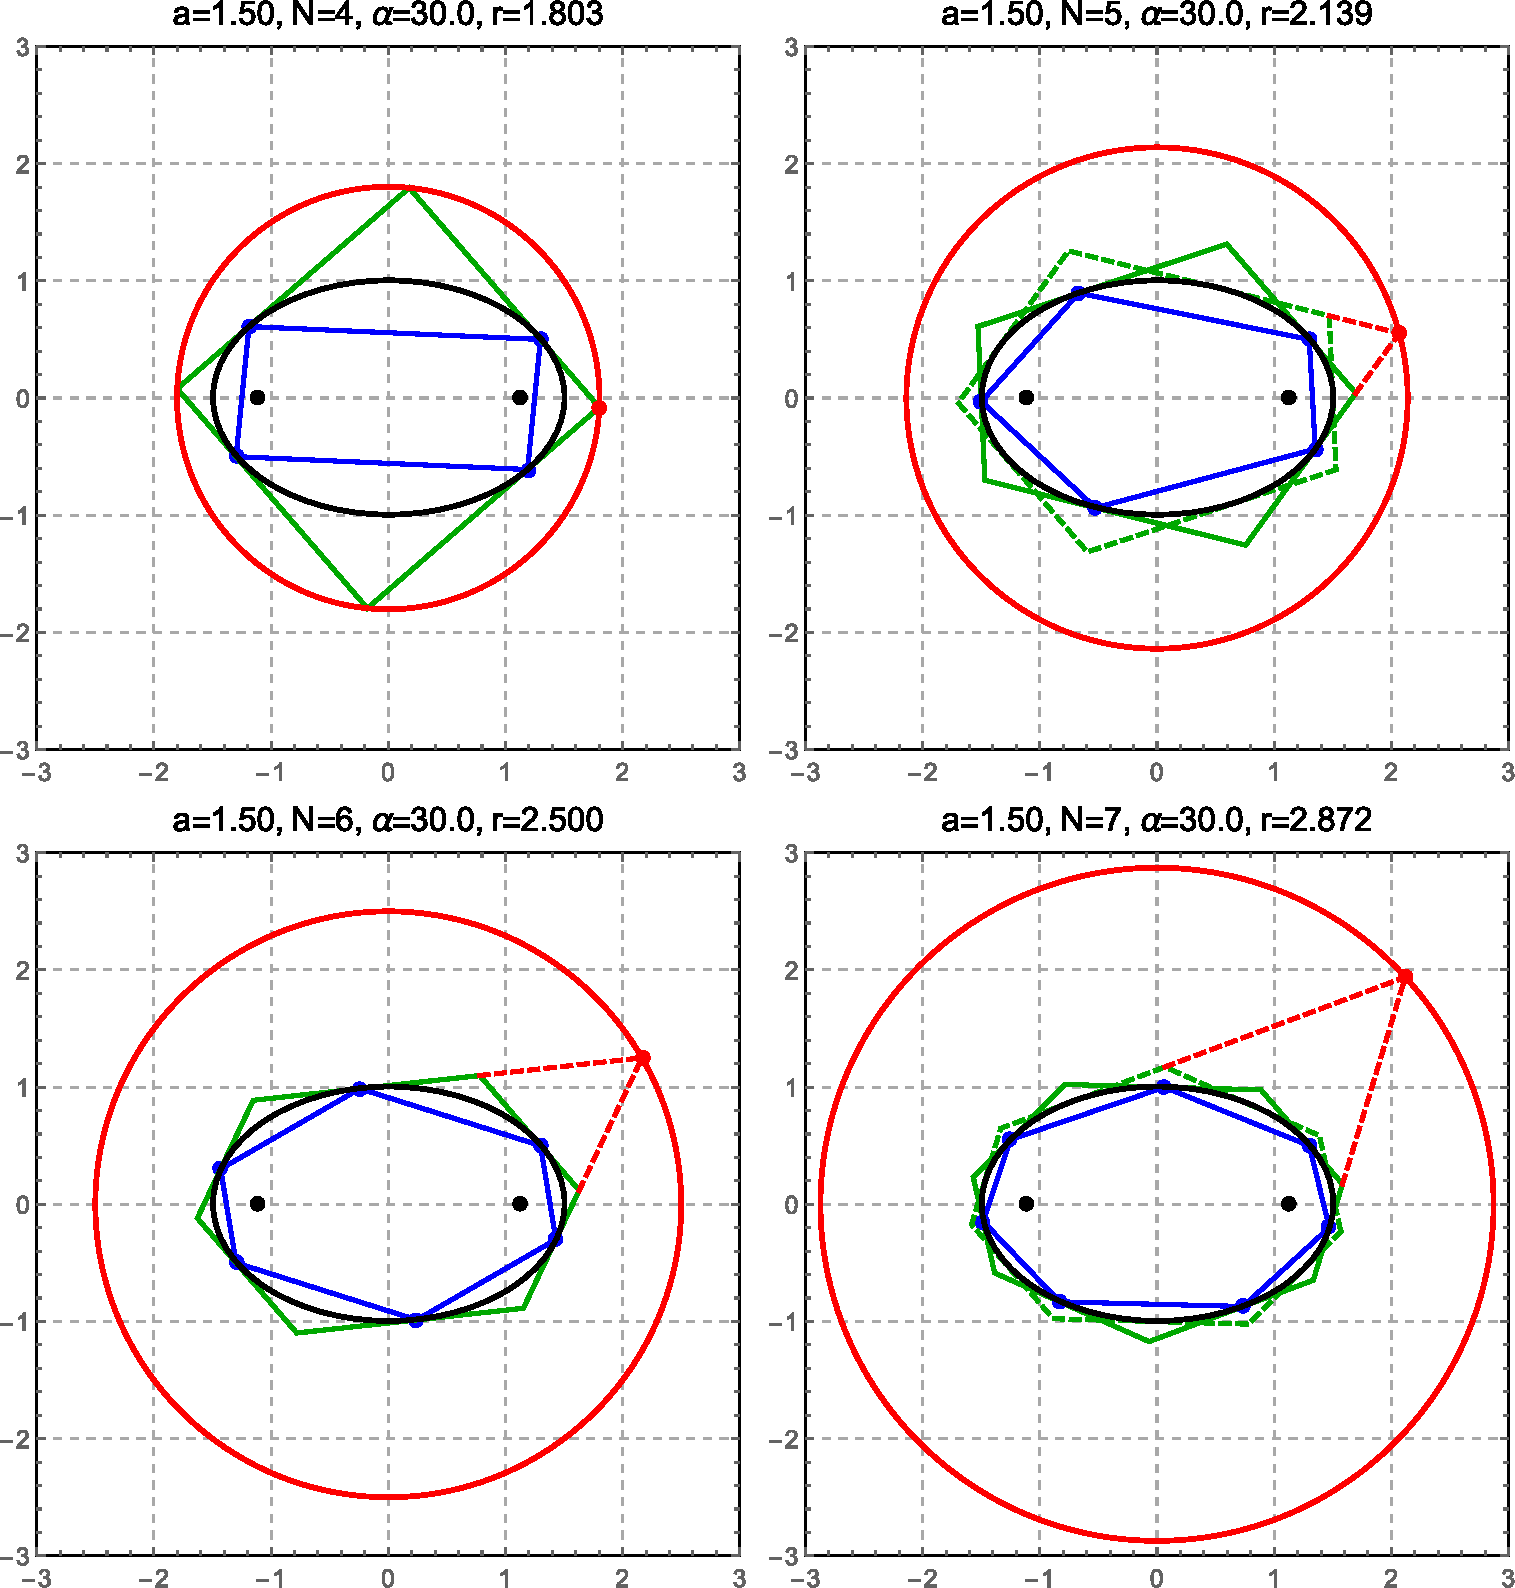
\includegraphics[width=\textwidth]{pics/0180_circ_grid.pdf}
    \caption{The loci of the intersection of an edge of the Tangential polygon with its reflection about the Billiard's center is a stationary circle for all $N$.}
    \label{fig:gen-circ-grid}
\end{figure}

\subsection{Summary}

The generalizations to $N>3$ found in this section are summarized on Table~\ref{tab:generalize}.

\begin{table}[H]
\caption{Generalizations of $N=3$ Invariants to $N>3$. Below $\theta_i,A,E_i$ refer to internal angle, area, or edge of the orbit polygon. When primed, they refer to the Tangential Polygon quantities. As before, $\delta=\sqrt{a^4+a^2-1}$.}
\label{tab:generalize}
$$
\begin{array}{r|c|c}
N=3~\mbox{Invariant} & N=3\,\mbox{Formula} & N\geq3\,\mbox{Invariant}  \\
\hline
\mbox{Perimeter L}&\frac{2(\delta+a^2+1)\sqrt{2\delta-a^2-1}}{a^2-1}&\mbox{Perimeter L}\\
\mbox{Angular Momentum}\,\gamma&\frac{\sqrt{2\delta-a^2-1}}{a^2-1}&\mbox{Angular Momentum}\\
\mbox{Mittenpunkt}\,X_9 & O & \mbox{Tang. medians meet at}\,O \\[5pt]
\frac{r}{R}=-1+\sum_{i=1}^3{\cos\theta_i} & \frac{2(\delta-1)}{(a^2-1)(\delta+a^2)} & \sum_{i=1}^N{\cos\theta_i} \\[5pt]
\prod_{i=1}^{3}{\cos\theta_i'} & \frac{r}{4R} & \prod_{i=1}^N{\cos\theta_i'} \\[5pt]
A'/A & \frac{2R}{r} & \forall{N}\mbox{ odd},A'/A\\[5pt]
\mbox{Radius of Cosine Circle }r^* &
    \frac{\sqrt{3}}{3}\sqrt{2\delta+a^2+1} & \mbox{Radius of }\,E'_i\cap-E'_{i+1},\,r^*=\frac{1}{\gamma}
\end{array}
$$
\end{table}